\documentclass[english]{beamer}

% Packages
\usepackage[utf8]{inputenc}
\usepackage[margin=1in]{geometry}
\usepackage{amssymb}
% PDF metadata
\usepackage[pdftex]{hyperref}
% For figure alignment
\usepackage{float}
% For colored text
\usepackage{xcolor}
% For SI unit notation
\usepackage{siunitx}
% For diagrams
\usepackage{tikz}
\usetikzlibrary{arrows.meta}
\usetikzlibrary{patterns.meta}
\usetikzlibrary{positioning}
\tikzset{>={Stealth[length=2mm]}}
% For citations
\usepackage[backend=biber]{biblatex}
% Better quotations
\usepackage[style=english]{csquotes}
% Language and localization
\usepackage{babel}
% Fix special characters
\usepackage[T1]{fontenc}


% Misc settings
% Remove indentation
\setlength{\parindent}{0in}
% Set paragraph spacing
\setlength{\parskip}{12pt}


% Macros
% Mark placeholder fields
\newcommand{\todo}[1][TODO]{{\color{red}#1}}

\hypersetup{
	pdftitle = {%
		Efficient CNN Accelerators on FPGAs
	},
	pdfauthor = {Clarity Shimoniak},
	pdfsubject = {EE 243 Project Presentation},
	pdfkeywords = {%
		computer vision, convolutional neural network, CNN, FPGA, Xilinx,
		Lattice, MNIST
	},
}

\addbibresource{fpga.bib}
\addbibresource{models.bib}
\addbibresource{related.bib}


\begin{document}

\title{Efficient CNN Accelerators on FPGAs}
\subtitle{EE 243 Final Project}
\author{Clarity Shimoniak}
\date{Spring 2024}
\frame{\titlepage}


\begin{frame}
\frametitle{Problem Statement and Motivation}
\begin{itemize}
	\item FPGA accelerators are promising for embedded applications where GPUs
	are unavailable.
	\item Depthwise-separable convolutions are key to the efficiency of
	MobileNet\supercites{mobilenetv1}{mobilenetv2} \&
	EfficientNet\supercite{efficientnet}.
	\item Existing FPGA accelerators do not implement them efficiently.
	\item Most FPGA accelerators do not publicly release code.
	\begin{itemize}
		\item All rely on expensive, proprietary Altera or Xilinx boards.
	\end{itemize}
\end{itemize}
\end{frame}


\begin{frame}
\frametitle{Framework Overview Figure}
\begin{figure}
	\centering
	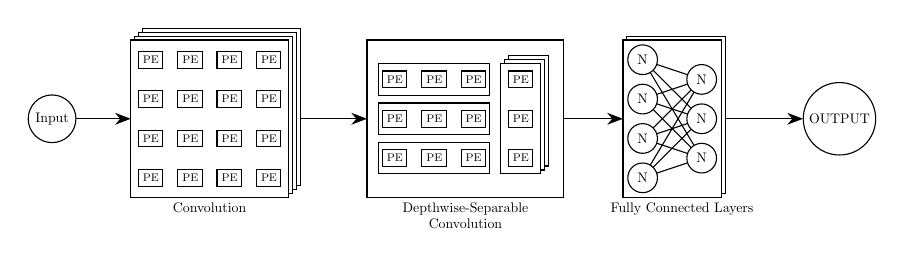
\begin{tikzpicture}[
	scale=0.5, transform shape,
	endpoint/.style = {
		circle, draw
	},
	pe/.style = {
		rectangle, draw,
		align=center,
		text width=11pt,
		font=\footnotesize
	},
	neuron/.style = {
		circle, draw,
		align=center,
		text width=10pt
	},
	label/.style = {
		anchor=north,
		align=center,
		text width=4cm
	}
]
	\node[endpoint] (in) at (0, 0) {Input};
	% Convolution Engine
	\node[label] at (4, -2) {Convolution};
	\foreach \i in {3,...,0} {
		\draw[fill=white] ({2 + \i/10}, {-2 + \i/10})
			rectangle ++(4, 4);
	}
	\foreach \x in {2,...,5} {
		\foreach \y in {-2,...,1} {
			\node[pe] at ({\x+0.5}, {\y+0.5}) {PE};
		}
	}
	% DSCV Engine
	\node[label] at (10.5, -2) {Depthwise-Separable Convolution};
	\draw[fill=white] (8, -2) rectangle ++(5, 4);
	% Depthwise
	\foreach \y in {-2,...,0} {
		\draw (8.3, {\y+0.6}) rectangle ++(2.8, 0.8);
		\foreach \x in {8,...,10} {
			\node[pe] at ({\x+0.7}, {\y+1}) {PE};
		}
	}
	% Pointwise
	\foreach \i in {2,...,0} {
		\draw[fill=white] ({11.4 + \i/10}, {-1.4 + \i/10})
			rectangle ++(1, 2.8);
	}
	\foreach \y in {-2,...,0} {
		\node[pe] at (11.9, {\y+1}) {PE};
	}
	% FC Layers
	\node[label] at (16, -2) {Fully Connected Layers};
	\foreach \i in {1,...,0} {
		\draw[fill=white] ({14.5 + \i/10}, {-2 + \i/10})
			rectangle ++(2.5, 4);
	}
	\node[neuron] (fc1a) at (15, -1.5) {N};
	\node[neuron] (fc1b) at (15, -0.5) {N};
	\node[neuron] (fc1c) at (15, 0.5) {N};
	\node[neuron] (fc1d) at (15, 1.5) {N};
	\node[neuron] (fc2a) at (16.5, -1) {N};
	\node[neuron] (fc2b) at (16.5, -0) {N};
	\node[neuron] (fc2c) at (16.5, 1) {N};
	\draw (fc1a) -- (fc2a);
	\draw (fc1b) -- (fc2a);
	\draw (fc1c) -- (fc2a);
	\draw (fc1d) -- (fc2a);
	\draw (fc1a) -- (fc2b);
	\draw (fc1b) -- (fc2b);
	\draw (fc1c) -- (fc2b);
	\draw (fc1d) -- (fc2b);
	\draw (fc1a) -- (fc2c);
	\draw (fc1b) -- (fc2c);
	\draw (fc1c) -- (fc2c);
	\draw (fc1d) -- (fc2c);
	%
	\node[endpoint] (out) at (20, 0) {OUTPUT};
	% Stage connections
	\draw[->] (in) -- ++(2, 0);
	\draw[->] (6.3, 0) -- ++(1.7, 0);
	\draw[->] (13, 0) -- ++(1.5, 0);
	\draw[->] (17.1, 0) -- (out);
\end{tikzpicture}

\end{figure}
\begin{columns}
	\column[t]{0.5\linewidth}
	\begin{itemize}
		\item Similar to early MobileNet stage.
		\item Trained with PyTorch on Colab.
		\begin{itemize}
			\item $\SI{81}{\percent}$ accuracy on CIFAR10.
		\end{itemize}
	\end{itemize}
	\column[t]{0.5\linewidth}
	\begin{itemize}
		\item Each convolution layer is followed by a ReLu and MaxPool.
		\item Converted to 8-bit fixed point for Verilog.
	\end{itemize}
\end{columns}
\end{frame}


\begin{frame}
\frametitle{Methodology}
\begin{columns}
	\column{0.8\linewidth}
	\begin{itemize}
		\item Create a minimal model with a similar structure to MobileNet.
		\begin{itemize}
			\item Only open-source FPGA MobileNet
			accelerator\supercite{solovyev2019mobilenet} is dependent on
			proprietary \$700 board.
			\item Remove as layers and channels as possible while maintaining high
			accuracy on a popular dataset.
		\end{itemize}
		\item Use the DPU architecture proposed by
		\citeauthor{mobilenet2019fpga}\supercite{mobilenet2019fpga}
		to accelerate it.
		\begin{itemize}
			\item Compare against an un-optimized architecture for the same network.
			\item Key improvement is separate depthwise-convolution engine.
		\end{itemize}
		\item Test synthesized model against images using Icarus Verilog.
	\end{itemize}
	\column{0.2\linewidth}
	\begin{figure}
		\centering
		\begin{figure}
	\centering
	\begin{tikzpicture}[
		scale=0.6, transform shape,
		endpoint/.style = {
			circle, draw
		},
		layer/.style = {
			rectangle, draw,
			align=center,
			text width=0.8in
		}
	]
		\node[endpoint] (in) {Input};
		\node[layer, below=of in] (conv1) {Convolution};
		\node[layer, below=of conv1] (conv2)
			{Depthwise-Separable Convolution};
		\node[layer, right=1.5cm of in] (fc1) {Linear 1};
		\node[layer, below=of fc1] (fc2) {Linear 2};
		\node[endpoint, below=of fc2] (out) {Output};
		\draw[->] (in) -- (conv1);
		\draw[->] (conv1) -- (conv2);
		\draw[->] (conv2) --
			($ (conv2) !0.5! (conv2 -| fc1)$) coordinate(low)
			-- (fc1 -| low) -- (fc1);
		\draw[->] (fc1) -- (fc2);
		\draw[->] (fc2) -- (out);
	\end{tikzpicture}
	\caption*{Simplified PyTorch Model}
\end{figure}

	\end{figure}
\end{columns}
\end{frame}


\begin{frame}
\frametitle{Experiments \& Results}
\end{frame}


\begin{frame}[allowframebreaks]
\frametitle{References}
\tiny\printbibliography
\end{frame}


\end{document}
